\documentclass[a4paper,xelatex,10pt,ja=standard]{bxjsarticle}

%% \XeLaTeXロゴ
\usepackage{metalogo}
%% subfigureのモダンな書き方のため
\usepackage[hang,small,bf]{caption}
\usepackage[subrefformat=parens]{subcaption}
\renewcommand{\subfigureautorefname}{\figureautorefname}
%% 箇条書き
\usepackage{enumerate}
%% bib
\usepackage[square,comma,numbers,sort&compress]{natbib}
%% ソースコードを貼り付けるため
\usepackage{listings, color}
%% 必須っぽい
\usepackage{amsmath, amssymb}
%% レイアウトのため
\usepackage{geometry, layout}
\geometry{top=2cm, bottom=2cm, left=1.5cm, right=1.5cm, includefoot}
%% リンクを貼るため
%% \usepackage[pdfborder={0 0 0}]{hyperref}
\usepackage[pdfborder={0 0 0}, colorlinks=true, pdfencoding=auto]{hyperref}
\newcommand*{\fullref}[1]{\hyperref[{#1}]{\autoref*{#1} \nameref*{#1}}}
\hypersetup{bookmarks=true,
        bookmarksnumbered=true,
        hidelinks,
        setpagesize=false,
        pdfauthor={EisokuKuroiwa}}

\author{Eisoku Kuroiwa}

\hypersetup{pdftitle={メモ},
        pdfsubject={memo},
        pdfkeywords={memo}}

\title{{\XeLaTeX}で日本語文書を書くときのメモ}

\begin{document}
\maketitle

参考文献テスト\cite{test}

以下で構成される

\begin{enumerate}
  \item \fullref{sec:no1}
  \item \fullref{sec:no2}
  \item \fullref{sec:no3}
\end{enumerate}

\section{{\TeX}で日本語の文章を書くときに気をつけること} \label{sec:no1}

処理系やドキュメントクラスなど色々あるが,確認事項としては,

\begin{enumerate}
 \item 日本語用ドキュメントクラスを使っているか
 \item 日本語とEnglishの間に「四分アキ」はあるか
 \item 日本語フォントは埋め込まれているか
\end{enumerate}

くらいがあるっぽい.
また,{\TeX}Liveは2010以降でないと日本語がutf-8で扱えないので,
Ubuntu14.04くらいからが良い.

\subsection{日本語用ドキュメントクラス}

まず,使用するドキュメントクラスが日本語用である必要がある.
理由は,日本語組版固有のスタイルがあるからで,それはそんなものかなという気がする.

最初にjarticleが作られたが,
規格に合っていなかったみたいでjsarticleが作られて,
jsarticleがplatexに強く依存していて他の処理系で使えなかったのでbxjsarticleが作られた,という流れ.
この文章はbxjsarticleを使っている.
なぜなら,platexやuplatexではなくて,xelatexを使いたかったから.
その理由は,latexrunを使いたかったから.
latexrunを使いたかったのは,出力を見やすくしてくれるから.

\subsection{四分アキ}

「CやC++では」,と書いたときに,日本語と英語との境目にスペースを入れるのが美しいらしく,そうなっているかどうか.
ちなみに,2016/02/15,Ubuntu14.04,bxjsarticleはgithubの最新の段階では,pdflatexを使うと四分アキが出来ず,xelatex / lualatexは四分アキが出来ていたが,lualatexよりもxelatexの方がビルドが早かったので,xelatexを使うことにした.

\subsection{フォントの埋め込み}
platexとdvipdfmxを組み合わせていた時は,dvipdfmxの-fオプションでフォントマップを指定しないと埋め込まれない,ということがあったが,pdflatexとかxelatexとかは何もしなくても埋め込まれる.

pdffonts xxx.pdfで確認可能で,embの欄がyesとなっていればいい.

\section{図の挿入}\label{sec:no2}

platexとdvipdfmxを組み合わせていた時は,extrabbコマンドなどでbbファイルを作ってやる必要があったが,最近は勝手にやってくれるようになった.

画像までのパスを入力するだけで
\begin{enumerate}
 \item \autoref{fig:nowprinting}のようにpdf
 \item \autoref{fig:nowprinting_png}のようにpng
 \item \autoref{fig:normal_distribution}のようにeps
 \item \autoref{fig:normal_distribution_jpg}のようにjpg
\end{enumerate}
を埋め込むことが可能.
拡大してみるとベクター形式かどうかで綺麗さが変わることが分かる.

\begin{figure}[htbp]
  \centering
  \begin{minipage}[b]{0.3\columnwidth}
    \centering
    
\includegraphics[width=\columnwidth]{figs/nowprinting}
    \subcaption{pdfの参考例}
    \label{fig:nowprinting}
  \end{minipage}
  \begin{minipage}[b]{0.3\columnwidth}
    \centering
    
\includegraphics[width=\columnwidth]{figs/nowprinting_png}
    \subcaption{pngの参考例2}
    \label{fig:nowprinting_png}
  \end{minipage}
  \\
  \begin{minipage}[b]{0.4\columnwidth}
    \centering
    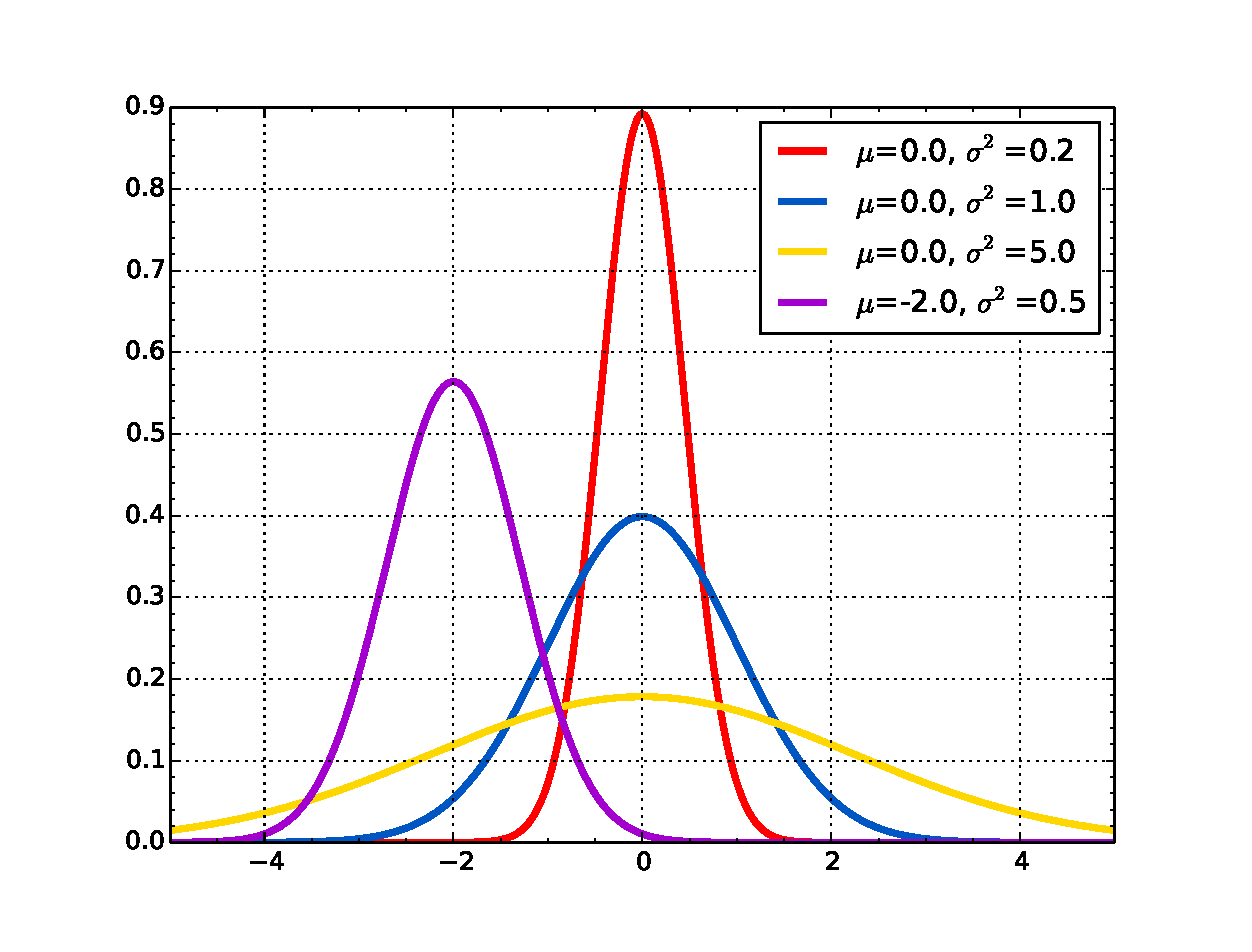
\includegraphics[width=\columnwidth]{figs/normal_distribution}
    \subcaption{epsの参考例}
    \label{fig:normal_distribution}
  \end{minipage}
  \begin{minipage}[b]{0.4\columnwidth}
    \centering
    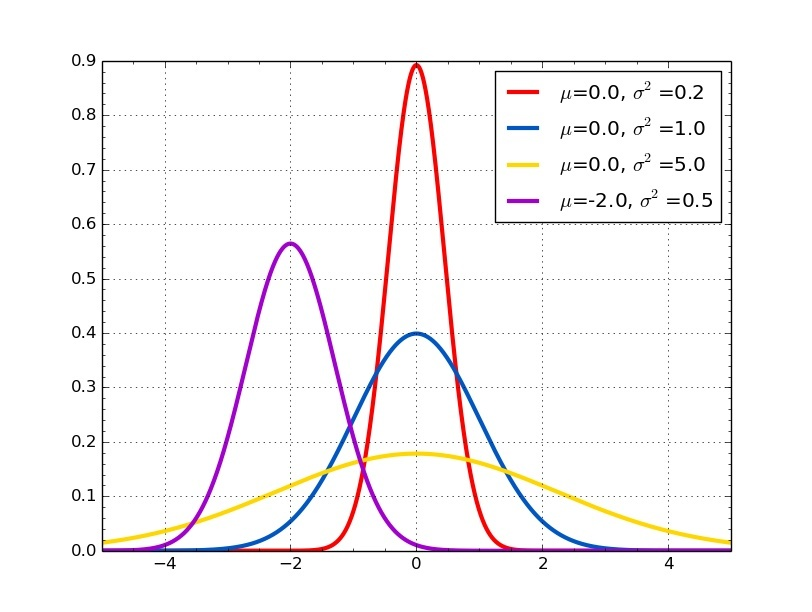
\includegraphics[width=\columnwidth]{figs/normal_distribution_jpg}
    \subcaption{jpgの参考例}
    \label{fig:normal_distribution_jpg}
  \end{minipage}
  \caption{図の参考例}
  \label{fig:example-of-figures}
\end{figure}

\autoref{listing:normal_distribution}のようにlistingを使えばソースコードを貼ることも可能.
こちらもパスを指定してあげるだけでOK.
本当はlistingではなくてmintedを使いたいが,pdflatexでないとmintedは使えないようなので,残念ポイント.

\lstinputlisting[language=Python, caption=normal\_distribution.py, label=listing:normal_distribution, numbers=left, showstringspaces=false,
  keywordstyle={\bfseries \color[cmyk]{1,0,0.1,0}},
  stringstyle={\ttfamily \color[cmyk]{0.5,0,1,0}},
  basicstyle=\ttfamily\small]{codes/normal_distribution.py}

\section{preambleについて}\label{sec:no3}
お決まりのusepackageやお決まりの余白などはまとめたい\footnote{\url{http://be.nucl.ap.titech.ac.jp/~sako/TeXmacro.pdf}}.

geometryパッケージ\footnote{\url{ftp://ftp.kddilabs.jp/CTAN/macros/latex/contrib/geometry/geometry.pdf}}で余白の設定ができる.

\layout


\bibliographystyle{unsrt}
%% \phantomsection
\setlength{\bibsep}{3pt}
\bibliography{bib}

\end{document}
